\documentclass[pdftex]{beamer}
\usetheme{Frankfurt}

% declare the path(s) where your graphic files are
% ../.. is the GeocronDocuments directory
\graphicspath{{../../images/external/location_routing/}{../../images/diagrams/}}
\DeclareGraphicsExtensions{.pdf,.png}

%some screwiness required to get the apalike bib style working
\usepackage{natbib}
\def\newblock{\hskip .11em plus .33em minus .07em}

\begin{document}

% This will make the icons next to bibitems appear as [#] instead of the silly article image
%deactivated since I'm using style apalike
%\setbeamertemplate{bibliography item}[text]

% Show the ToC at the start of each section, with the current section highlighted
\AtBeginSection[]
{
   \begin{frame}
        \frametitle{Roadmap}
        \tableofcontents[currentsection]
   \end{frame}
}

\title[Location routing]{Location-Based Routing}
\subtitle{An overview and possible directions for GeoCRON}
\author[K. Benson]{Kyle E. Benson}
\institute[UCI]{
  Department of Computer Science\\
  University of California, Irvine\\
  Irvine, California 92697\\[1ex]
  \texttt{kebenson@uci.edu}
}


\begin{frame}[plain]
	\titlepage
\end{frame}

% Breaking intro into its own part suppresses navigation bar info
\part{intro}

\begin{frame}{Introduction}

\begin{itemize}
	\item Traditional routing
	\begin{itemize}
		\item Unique address: IP, MAC, Peer ID, etc.
		\item Source routing: next hop address, neighbor index
		\item Local routing: distance-vector, link state, label-switching
	\end{itemize}
	
	\pause
	\item Why location information?
	\begin{itemize}
		\item Geocast: message all (or some) nodes in target region
		\item Latency: request from closer server, route locally when possible
		\item Congestion: confine route requests to smaller regions (MANETs)
		\item Energy: closer nodes need less radio power to reach
		\item Sensors: regional event detection, spatial querying
		\item Planning: paths (robots), surveillance cameras (focus on area target will appear next)
		\alert<3>{\item Recovery: avoid problematic areas of the network}
		\begin{itemize}
		\alert<3>{\uncover<3>{\item our primary interest!}}
		\end{itemize}
	\end{itemize}
\end{itemize}

\end{frame}

% % % % % % % % % % % % % % % % % % % % % % % % % % % % % % % % % % % % % % % % % %
\part{rest}

\begin{frame}{Roadmap}
	\tableofcontents
\end{frame}

\section{Location Service}

\begin{frame}{Location Service}
\begin{columns}
\begin{column}{.5\textwidth}

	\begin{itemize}
		\item Nodes have GPS
		\item But how to look up destination's location?
		\item Maintain global information \uncover<2->{\alert{easily outdated/inefficient}}
		\item<3-> Distribute load
		\begin{itemize}
			\item In \cite{Li:2000:SLS:345910.345931}, node updates \emph{location servers} (LS) throughout network
			\item Divide network into hierarchical grid
			\item LS's in 3 external grids at each level
			\item Lookup distance $<$ square LS co-resides in
		\end{itemize}
		
	\end{itemize}

\end{column}

\begin{column}{.5\textwidth}
\uncover<3->{
\begin{figure}
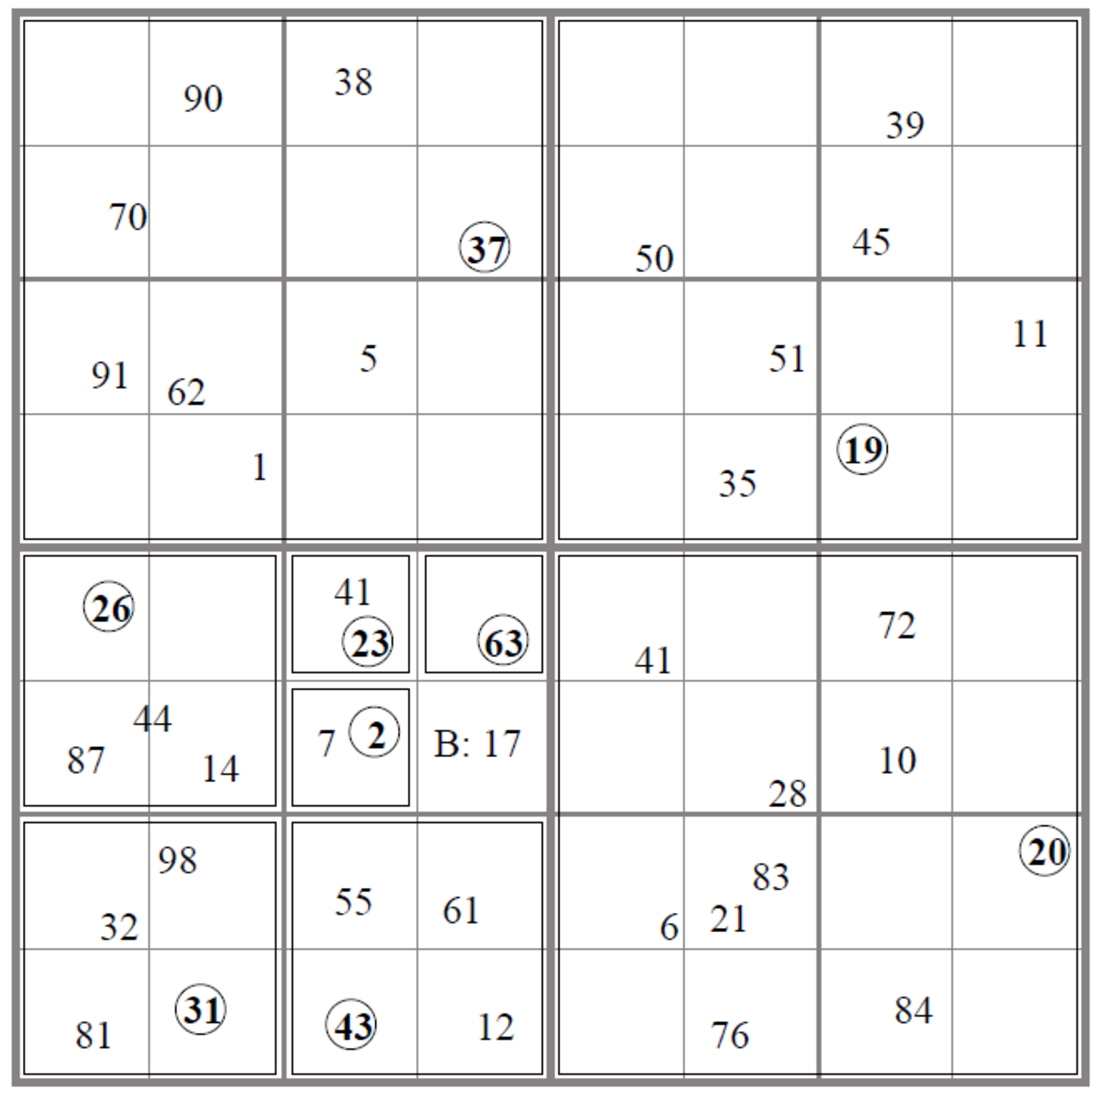
\includegraphics[width=\textwidth]{location_service}
\caption{Hierarchical grid with 4 order-i squares in order-i+1 square.}
\end{figure}}
\end{column}
\end{columns}
\end{frame}


\begin{frame}{Location Service for GeoCRON}
\begin{columns}
\begin{column}{.5\textwidth}

	\begin{itemize}
		\item Grid $\Leftrightarrow$ CSN's \emph{geocells}
		\item Location servers $\rightarrow$ sensor's overlay contacts
		\item Natural geographic diversity $\rightarrow$ more robust!
		\item Location servers hold address, NOT just location!
		\item Region ID $\leftarrow$ quad tree path
		\vspace{-12pt} %strange formatting here, maybe the arrows?
		\begin{itemize}
			\item \emph{ex:} $B$ at 203 (count like Cartesian plane)
		\end{itemize}
		\item Region similarity $\rightarrow$ prefix match region ID
	\end{itemize}

\end{column}

\begin{column}{.5\textwidth}
\begin{figure}
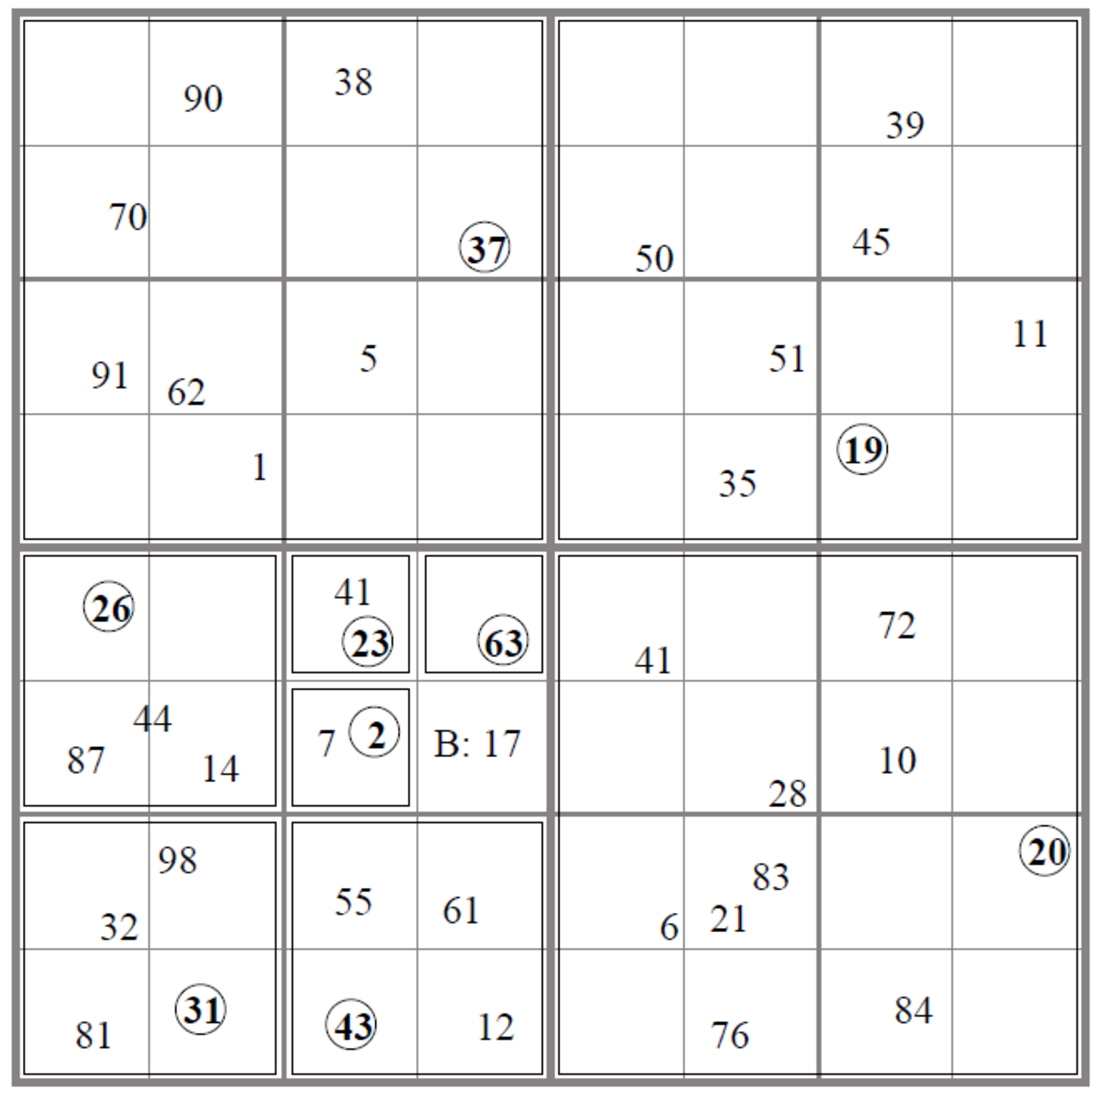
\includegraphics[width=\textwidth]{location_service}
\caption{Hierarchical grid closely resembles CSN's \emph{geocells}}
\end{figure}
\end{column}
\end{columns}
\end{frame}

% % % % % % % % % % % % % % % % % % % % % % % % % % % % % % % % % % % % % % % % % %

\section{Greedy Forwarding}


\begin{frame}{Greedy Forwarding}
\begin{columns}
\begin{column}{.5\textwidth}
\begin{itemize}
	\item Forward to next closest hop to destination
	\item What if no such neighbor?
	\begin{itemize}
		\item Reached local minimum
		\item \emph{Voids} in network 
		\item Solution: temporarily forward to farther hop
		\item Used by \cite{Ko98location-aidedrouting, 749282} with parameter $\delta$
		\item Forward if next hop distance $\leq$ previous distance + $\delta$
	\end{itemize}
\end{itemize}
\end{column}

\begin{column}{.5\textwidth}
\begin{figure}
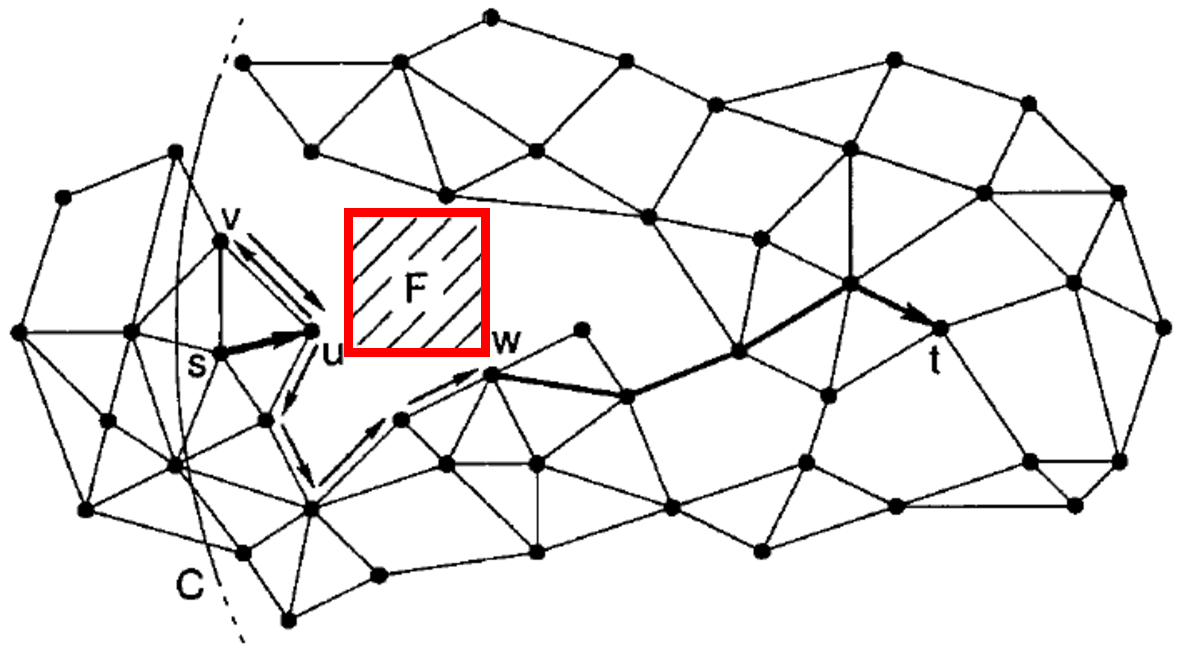
\includegraphics[width=\textwidth]{void}
\caption{A void in a network (roughly centered at F, outlined in red) may disrupt greedy forwarding}
\end{figure}
\end{column}
\end{columns}
\end{frame}


\begin{frame}{Greedy Forwarding in confined region}
\begin{columns}
\begin{column}{.5\textwidth}
\begin{itemize}
	\item In \cite{749282}, source defines a \emph{multicast region} and \emph{forwarding zone}
		\begin{itemize}
			\item Message delivered to all nodes in multicast region
			\item Defined as a rectangle, coordinates inside message
			\item Includes source, destination, plus error
			\item Message flooded within forwarding zone until target reached
		\end{itemize}
\end{itemize}
\end{column}

\begin{column}{.5\textwidth}
\begin{figure}
\centering
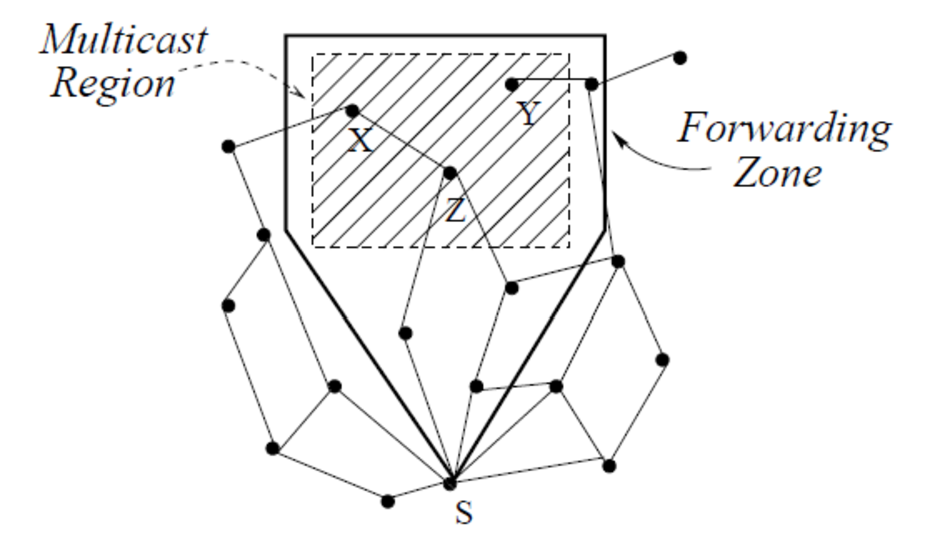
\includegraphics[width=\textwidth]{geocast_region}
\caption{Depiction of multicast region and forwarding zone}
\end{figure}
\end{column}
\end{columns}
\end{frame}


\begin{frame}{Greedy Forwarding further enhancements}
\begin{columns}
\begin{column}{.5\textwidth}
\begin{itemize}
	\item Adapt forwarding region at each hop \cite{749282}
		\begin{itemize}
			\item Intermediate (closer) nodes know topology better
			\item Change region shape
		\end{itemize}
	\item Adaptive technique may help GeoCRON
		\begin{itemize}
			\item Failure assumed close to sensors
			\item Message farther away $\rightarrow$\\ less chance of failures $\rightarrow$\\ routing region shrinks
		\end{itemize}
\end{itemize}
\end{column}

\begin{column}{.5\textwidth}
\begin{figure}
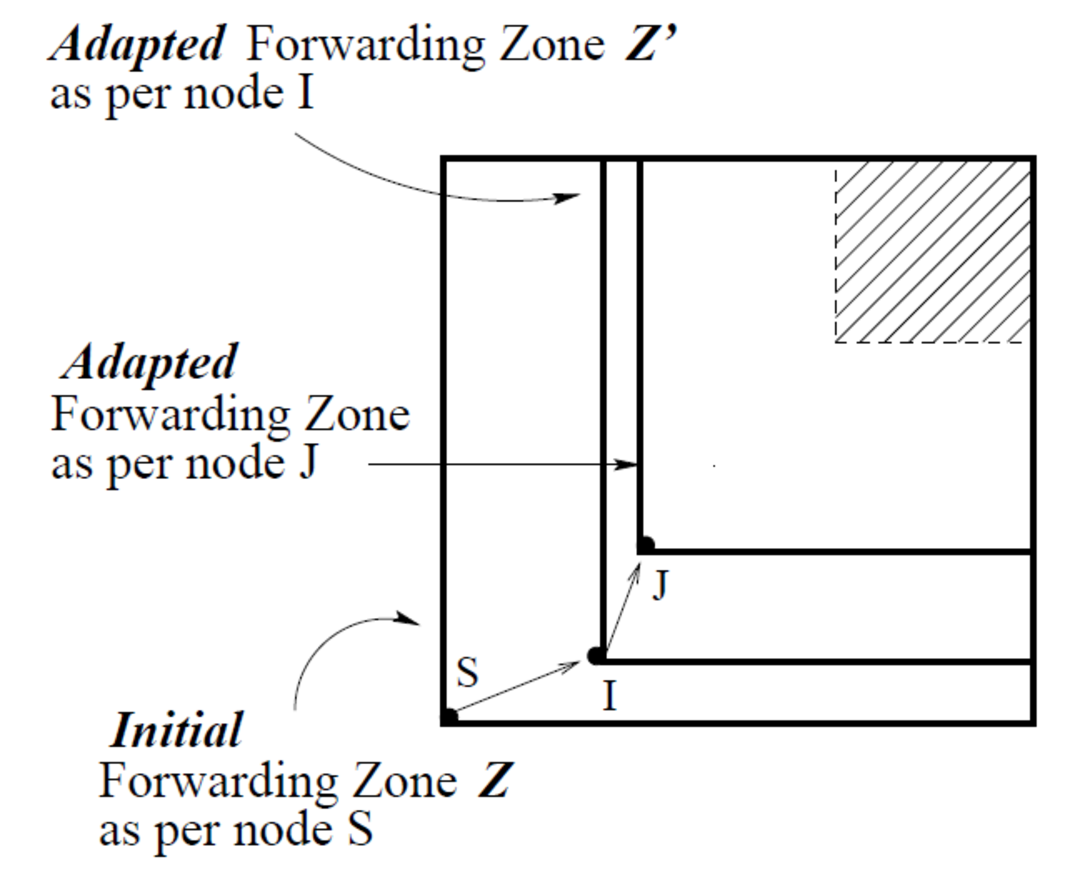
\includegraphics[width=\textwidth]{adaptive_geocast_region}
\caption{Depiction of adaptive multicast region and forwarding zone}
\end{figure}
\end{column}
\end{columns}
\end{frame}

% % % % % % % % % % % % % % % % % % % % % % % % % % % % % % % % % % % % % % % % % %

\section{Trajectory Routing}

\begin{frame}{Trajectory Routing}
\begin{columns}
\begin{column}{.5\textwidth}
	\begin{itemize}
		\item Introduced in \cite{Niculescu2003, Niculescu2004}, implemented in \cite{Yuksel2006}
		\item Message follows a curve
		\item Hybrid greedy/source routing
		\item Forward to neighbor furthest along curve
		\item Routes around voids, obstacles, etc.
		\item GeoCRON: identify failed regions $\rightarrow$ route around
	\end{itemize}
\end{column}
	
\begin{column}{.5\textwidth}
\begin{figure}
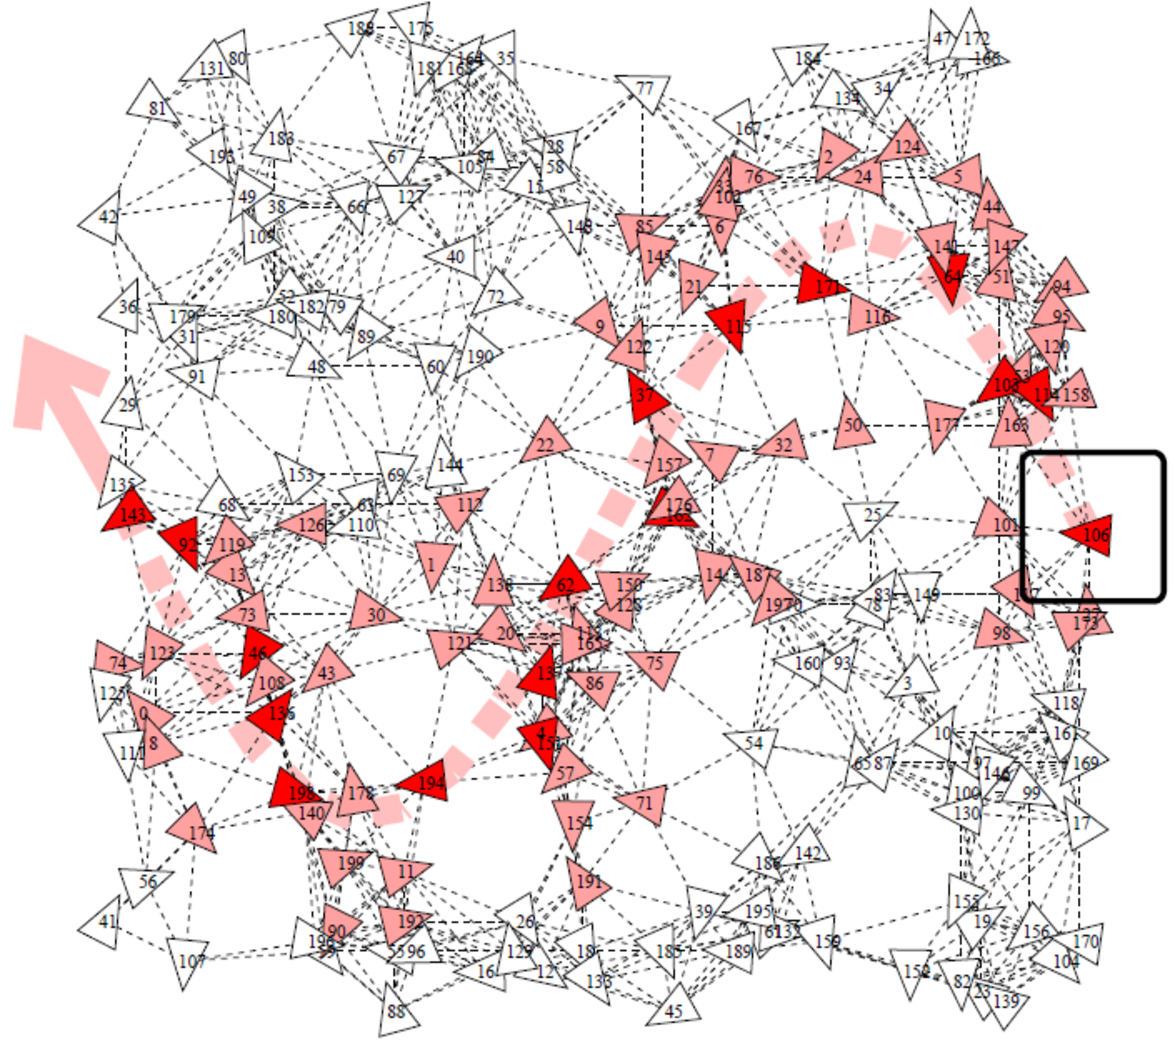
\includegraphics[width=\textwidth]{trajectory}
\caption{Forwarding along a trajectory}
\end{figure}
\end{column}
\end{columns}
\end{frame}

% % % % % % % % % % % % % % % % % % % % % % % % % % % % % % % % % % % % % % % % % %

\section{Geometric Routing}

\begin{frame}{Geometric Routing}
\begin{columns}
\begin{column}{.5\textwidth}
	\begin{itemize}
		\item Network topology $\rightarrow$ graph
			\begin{itemize}
				\item Vertices $=$ nodes
				\item Edges $=$ direct communication
			\end{itemize}
		\pause
		\item Graph geometry $\rightarrow$ forwarding
		\pause
		\item \emph{Compass routing} proposed \cite{Kranakis99compassrouting}
		\begin{itemize}
			\item \emph{Right-hand rule}
			\item Also called \emph{face routing}
			\item Also used in \cite{Kuhn2003, Kim:2005:GRM:1251203.1251219}
		\end{itemize}
\end{itemize}
\end{column}

\begin{column}{.5\textwidth}
\begin{figure}
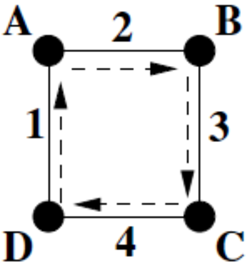
\includegraphics[width=.5\textwidth]{right_hand_rule}
\caption{The right-hand rule: forward packet along next counter-clockwise edge. Analogous to following the right hand wall in a maze.}
\end{figure}
\end{column}
\end{columns}
\end{frame}


\begin{frame}{Geometric Routing in GeoCRON}
\begin{columns}
\begin{column}{.5\textwidth}
	\begin{itemize}
		\item Overlay network $\rightarrow$ planar graph
		\item Faces large enough to avoid routing back to failed regions
		\item Intermediary makes routing decision, NOT source
\end{itemize}
\end{column}

\begin{column}{.5\textwidth}
\begin{figure}
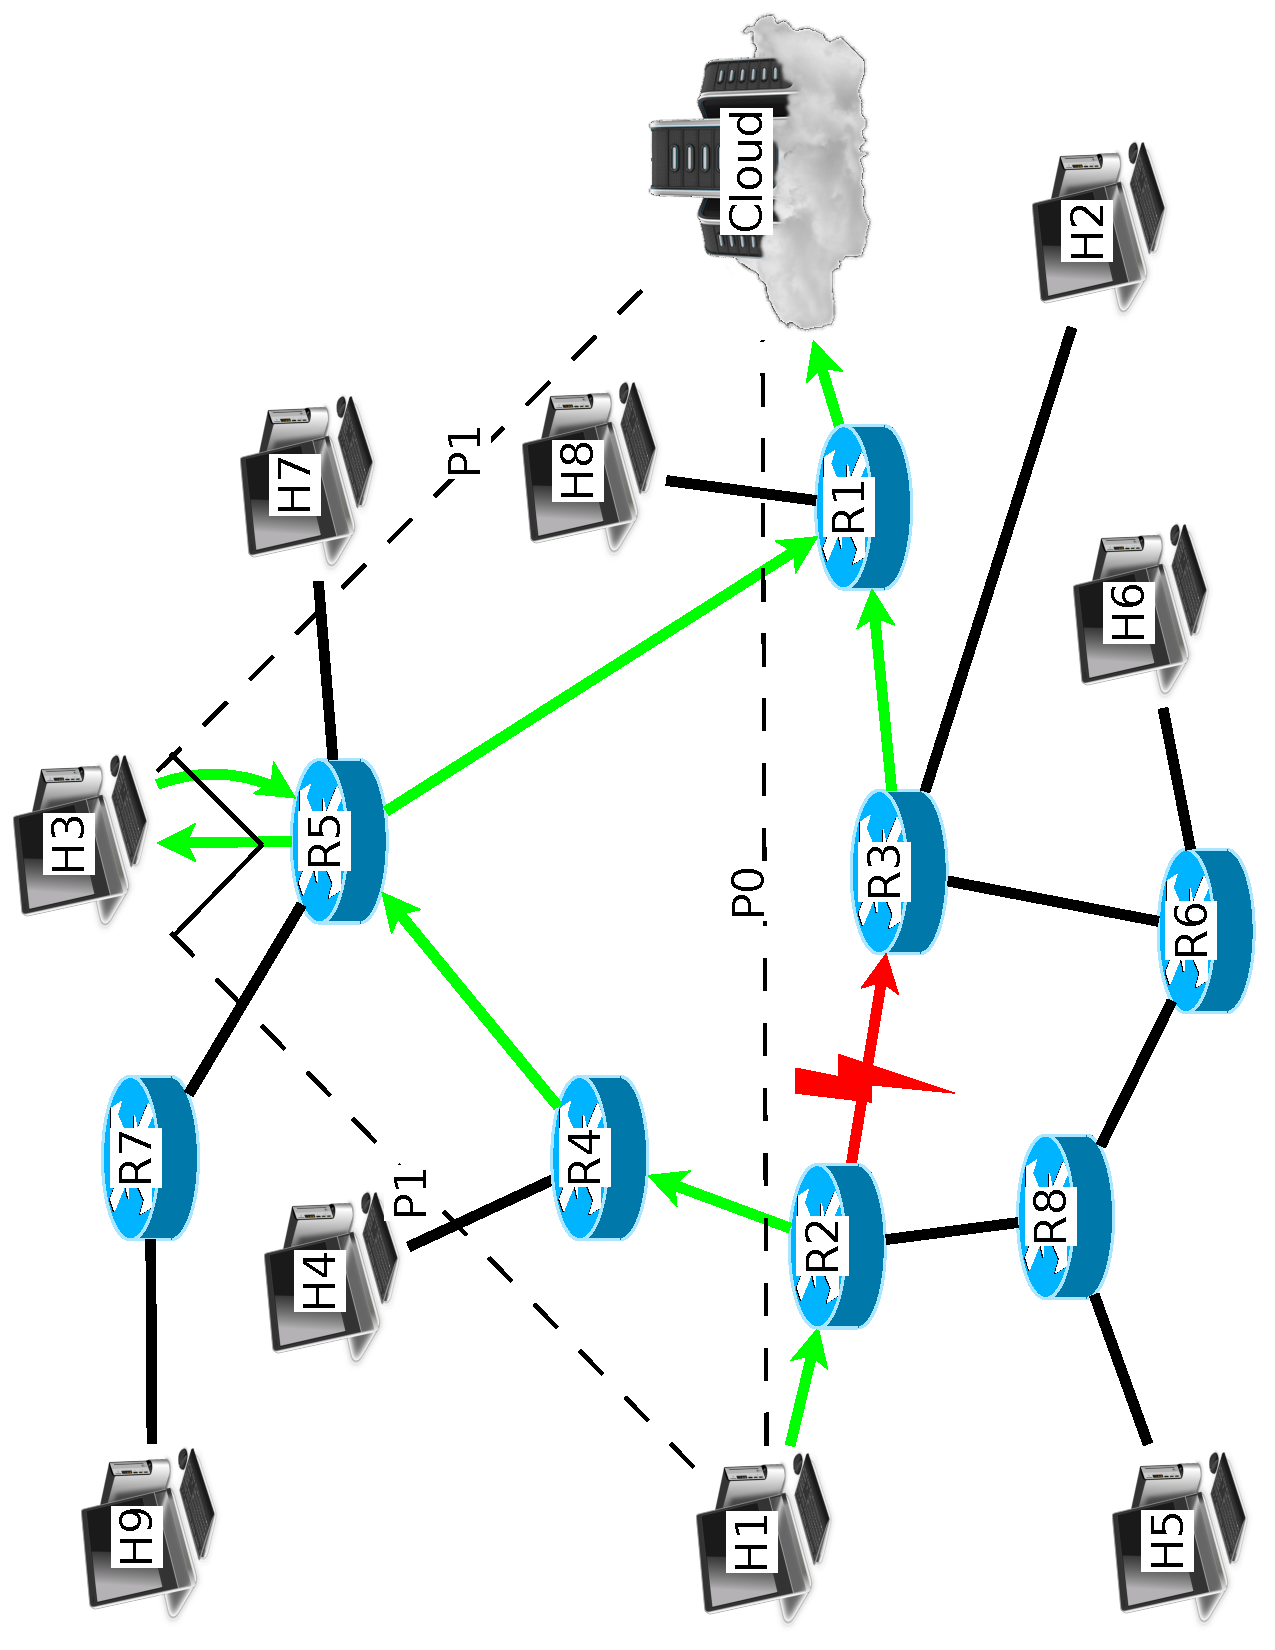
\includegraphics[height=\textwidth, angle=-90]{angular_path}
\caption{Apply right-hand rule to overlay paths.  Similar to Orthogonal Path Heuristic.}
\end{figure}
\end{column}
\end{columns}
\end{frame}
% % % % % % % % % % % % % % % % % % % % % % % % % % % % % % % % % % % % % % % % % %

\section{Clustering}

\begin{frame}
	\begin{itemize}
		\item GRID \cite{Liao01grid:a} divides network into squares
		\begin{itemize}
			\item Gateway chosen for each square
			\item Zone-based version of AODV to route
			\item Route requests confined to geographic region
		\end{itemize}
		\item In \cite{779923}, an inter-zone clustering protocol periodically run
		\begin{itemize}
			\item Updated with inter-zone links
			\item Destination's exact location within zone unknown $\rightarrow$ packet gets close enough
		\end{itemize}	
	\end{itemize}
\end{frame}


\begin{frame}{Clustering - LABAR}
\begin{columns}
\begin{column}{.5\textwidth}
\begin{itemize}
	\item LABAR \cite{Zaruba2003}
		\begin{itemize}
			\item GPS-enabled nodes $\rightarrow$ backbone G-nodes
			\item Nodes near G-nodes belong to a \emph{zone}
			\item G-nodes give sender vector towards intermediary zones
		\end{itemize}
\end{itemize}
\end{column}

\begin{column}{.5\textwidth}
\begin{figure}
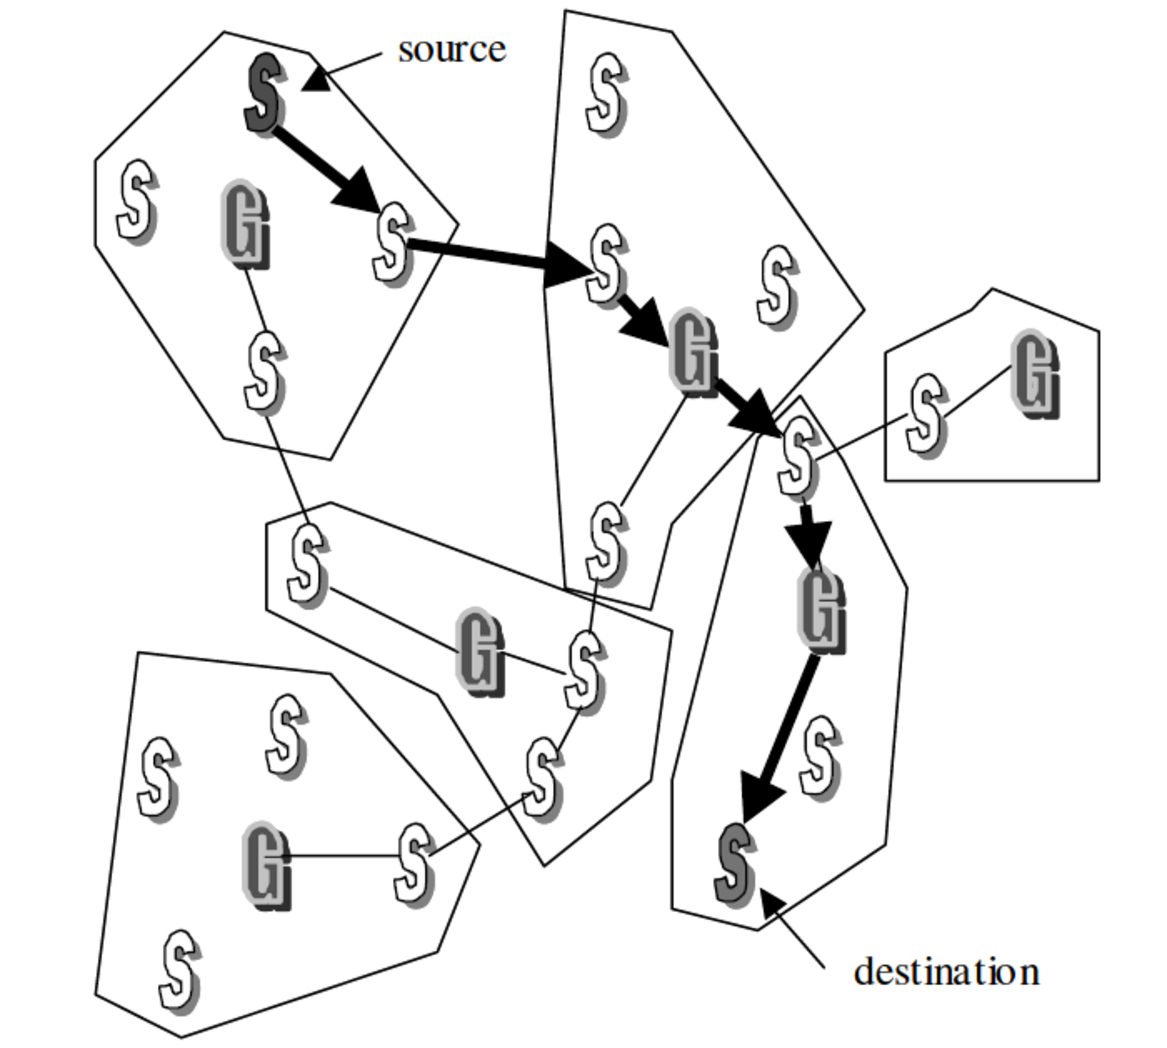
\includegraphics[width=\textwidth]{labar}
\caption{Routing in LABAR}
\end{figure}
\end{column}
\end{columns}
\end{frame}


\begin{frame}{Clustering in GeoCRON}
	\begin{itemize}
	\item Sensors clustered by region (city, geocell, etc.)
	\item More reliable node (or first to reach server) $\rightarrow$ clusterhead
	\item Sensors report to clusterhead
	\item Clusterhead forwards aggregate packets
	\begin{itemize}
		\item Data compression
		\item Paths overlap anyway $\rightarrow$ reduce local congestion
		\item Cluster aware of failures
		\item<2-> \alert{Problem:} increased latency if $>$ 1 overlay hop
		\item<3-> \alert{Problem:} what if clusterhead fails?
	\end{itemize}
	\end{itemize}
\end{frame}

% % % % % % % % % % % % % % % % % % % % % % % % % % % % % % % % % % % % % % % % % %

\section{Hybrid}

\begin{frame}{Hybrid}
\begin{itemize}
	\item In \cite{Kuhn2003, Huang2005, Karp2000}, greedy forwarding until \emph{void} reached
	\begin{itemize}
		\item \emph{Face routing} within a bounded region
		\item Enlarge bounded region if destination unreachable
		\item FAR \cite{Huang2005} introduced \emph{mobicast}: mobile geocast
		\begin{itemize}
			\item Application: mobile regional sensing
			\item \emph{Just in time} forwarding: packet arrives right before mobicast region
			\item Decreases \emph{lag time} (how long nodes hold data before mobicast region arrives)
		\end{itemize}
	\end{itemize}
	\item Such hybrid approaches necessary in GeoCRON
	\begin{itemize}
		\item Adaptability $\rightarrow$ resilience
		\item One technique may work well for some failures, not for others
		\item e.g. earthquake $\neq$ hurricane
	\end{itemize}
\end{itemize}
\end{frame}

% % % % % % % % % % % % % % % % % % % % % % % % % % % % % % % % % % % % % % % % % %

\section{Wired Overlay Routing}

\begin{frame}{Wired Overlay Routing - path choices}
\begin{columns}
\begin{column}{.5\textwidth}
\begin{itemize}
	\item Little work done in this context
	\item In \cite{Kim2010} overlay-based data dissemination is considered
	\item Overlay neighbors chosen to minimize distance between routers on path
	\item Intuition: geo-correlated failures affect nodes in proximity
	\item Improve path diversity
\end{itemize}
\end{column}

\begin{column}{.5\textwidth}
\begin{figure}
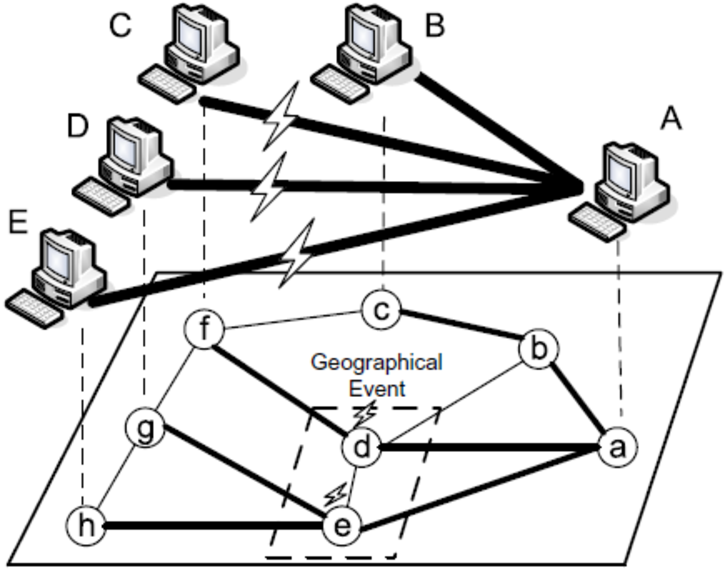
\includegraphics[width=\textwidth]{geo_failures_kyungbaek}
\caption{Different overlay links may share the same underlay links/nodes}
\end{figure}
\end{column}
\end{columns}
\end{frame}


\begin{frame}{Wired Overlay Routing - regional trees}
\begin{columns}
\begin{column}{.5\textwidth}
\begin{itemize}
	\item Concept of \emph{responsible region tree (RRTree)} used in \cite{6424865}
	\item Similarly to GRID, regions organized hierarchically
	\item RRTree nodes' region $=$ childrens'
	\item Each has emph{region hopping table} to contact non-adjacent regions
	\item Route tree in O(logn)
	\item Conjugate regions $\rightarrow$ geographically diverse $\rightarrow$ maintain external communication
	
\end{itemize}
\end{column}

\begin{column}{.5\textwidth}
\begin{figure}
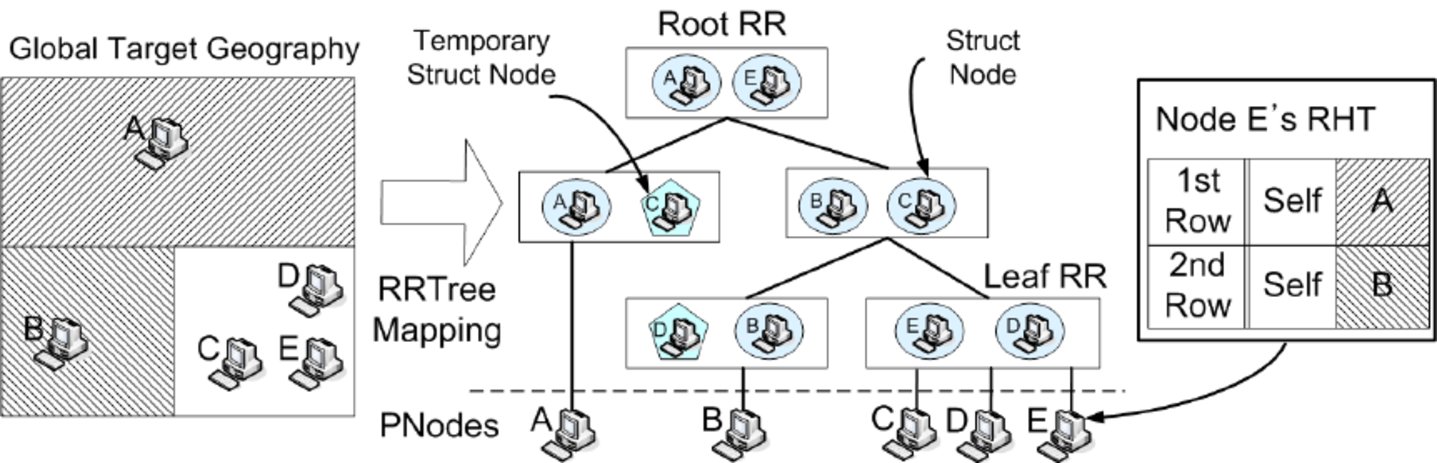
\includegraphics[width=\textwidth]{gsford_rrtree}
\caption{Depiction of GSFord's RRTree, RHT, and target geography}
\end{figure}
\begin{figure}
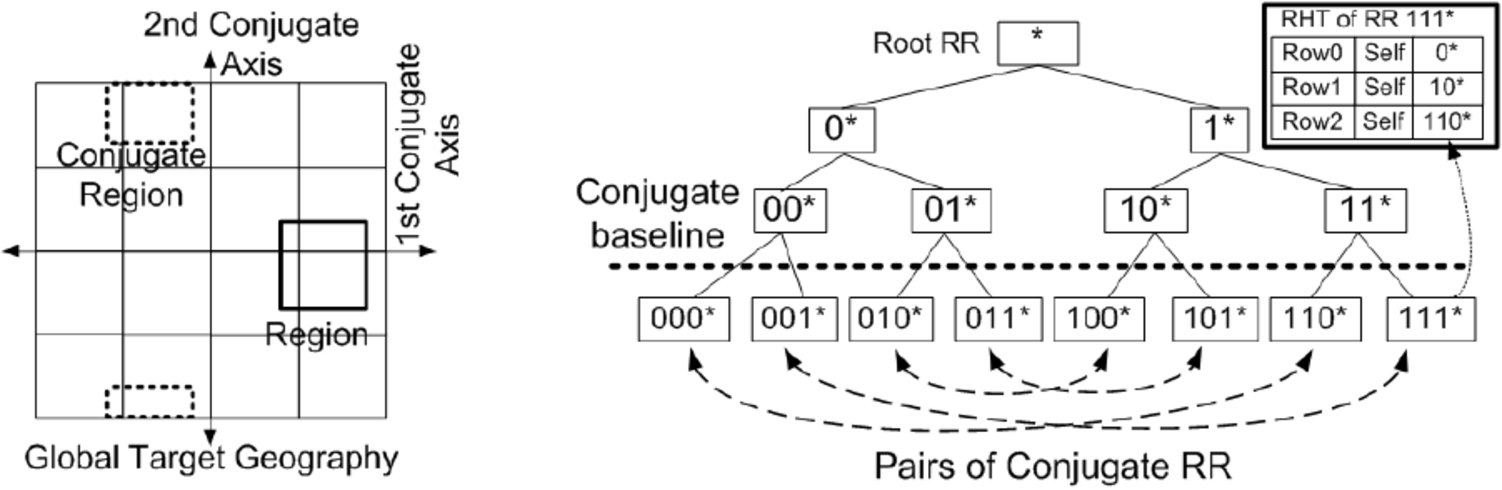
\includegraphics[width=\textwidth]{gsford_conjugate_region}
\caption{Depiction of GSFord's conjugate regions}
\end{figure}
\end{column}
\end{columns}
\end{frame}

% % % % % % % % % % % % % % % % % % % % % % % % % % % % % % % % % % % % % % % % % %

\part{bib}

\begin{frame}[allowframebreaks]{References}
\bibliographystyle{apalike}
% argument is your BibTeX string definitions and bibliography database(s)
\bibliography{IEEEabrv,location_routing}
\end{frame}

\end{document}
